\section{Eksplorasi Data}
\subsection{Statistika Deskriptif}
Sebelum melakukan proses pemodelan dengan metode ARIMA dan STARIMA, langkah pertama yang dilakukan adalah melakukan eksplorasi data yaitu dengan statistika deskriptif. Tujuannya untuk memahami karakteristik dasar data seperti tren, musiman, serta variabilitas yang terjadi. Melalui analisa deskriptif, diperoleh gambaran umum mengenai perilaku data yang akan dimodelkan.

\begin{table}[H]
    \centering
    \caption{Statistika Deskriptif}
    \label{table:statistik_deskriptif}
    \begin{tabular}{lccccc}
        \toprule
        \textbf{Statistik} & \textbf{Barat} & \textbf{Selatan} & \textbf{Tengah} & \textbf{Timur} & \textbf{Utara} \\
        \midrule
        Count & 3653.000000 & 3653.000000 & 3653.000000 & 3653.000000 & 3653.000000 \\
        Mean  & 5.843041    & 5.920063    & 5.919724    & 5.206096    & 5.842067    \\
        Min   & 0.000000    & 0.000000    & 0.000000    & 0.000000    & 0.000000    \\
        25\%  & 0.090000    & 0.000000    & 0.020000    & 0.000000    & 0.120000    \\
        50\%  & 1.650000    & 0.780000    & 1.370000    & 0.600000    & 2.010000    \\
        75\%  & 7.520000    & 6.560000    & 7.630000    & 6.400000    & 8.030000    \\
        Max   & 308.380000  & 366.490000  & 318.680000  & 195.030000  & 249.460000  \\
        Std   & 11.013619   & 13.287137   & 11.868456   & 10.058238   & 10.116447   \\
        \bottomrule
    \end{tabular}
\end{table}

Tabel~\ref{table:statistik_deskriptif} menyajikan hasil analisis statistika deskriptif curah hujan pada lima wilayah Kota Surabaya, yaitu Barat, Selatan, Tengah, Timur, dan Utara. Berdasarkan tabel tersebut, jumlah data pengamatan pada masing-masing wilayah adalah 120 observasi, yang menunjukkan bahwa seluruh wilayah memiliki panjang deret waktu yang sama sepanjang periode penelitian.

Secara umum, nilai rata-rata (mean) curah hujan di kelima wilayah berkisar antara 5,20 hingga 5,92 mm, yang menunjukkan bahwa intensitas curah hujan harian di Kota Surabaya relatif seragam antar wilayah. Wilayah Tengah (5,92 mm) memiliki rata-rata curah hujan tertinggi, diikuti oleh Selatan (5,92 mm) dan Barat (5,84 mm), sedangkan wilayah Timur (5,21 mm) mencatat rata-rata terendah.

Nilai minimum pada seluruh wilayah adalah 0 mm, yang menandakan adanya hari-hari tanpa hujan selama periode pengamatan. Sementara itu, nilai maksimum menunjukkan variasi yang cukup tinggi, di mana curah hujan ekstrem tertinggi tercatat di wilayah Selatan (366,49 mm), diikuti oleh Tengah (318,68 mm) dan Barat (308,38 mm). Hal ini menunjukkan bahwa wilayah bagian selatan Surabaya cenderung mengalami intensitas hujan ekstrem lebih besar dibandingkan wilayah lainnya.

Berdasarkan nilai median (50\%), sebagian besar wilayah memiliki nilai tengah curah hujan antara 0,6 hingga 2,0 mm, yang berarti sebagian besar hari dalam periode pengamatan memiliki curah hujan rendah hingga sedang. Nilai kuartil atas (75\%) menunjukkan bahwa 75\% data memiliki curah hujan di bawah 7–8 mm, sedangkan sisanya mewakili kejadian hujan intensitas tinggi.

Nilai simpangan baku (standar deviasi) berkisar antara 10,05 hingga 13,28, yang mengindikasikan adanya variasi curah hujan yang cukup besar antar waktu. Wilayah Selatan memiliki standar deviasi tertinggi (13,29), yang menandakan fluktuasi curah hujan paling tinggi, sedangkan wilayah Timur menunjukkan variasi paling rendah (10,06).

Secara keseluruhan, analisis deskriptif ini menunjukkan bahwa curah hujan di lima wilayah Kota Surabaya memiliki pola sebaran yang relatif serupa, namun dengan tingkat variabilitas dan intensitas ekstrem yang berbeda antar wilayah. Temuan ini mendukung perlunya analisis spasio-temporal lanjutan menggunakan model STARIMA untuk menangkap hubungan dinamis antar wilayah dan antar waktu.

\subsection{Pola Curah Hujan Kelima Wilayah di Surabaya}
Data yang digunakan adalah data curah hujan hasil dari pengamatan satelit NASA POWER pada lima titik wilayah di Kota Surabaya yaitu Utara, Selatan, Timur, Tengah dan Barat selama periode 1 Januari 2025 hingga 31 Desember 2024. Data curah hujan nya memiliki satuan mm/hari dan kemudian dilakukan aggregasi menjadi rata-rata bulanan agar dapat menggambarkan tren musiman jangka panjang.

\begin{figure}[H]
    \centering
    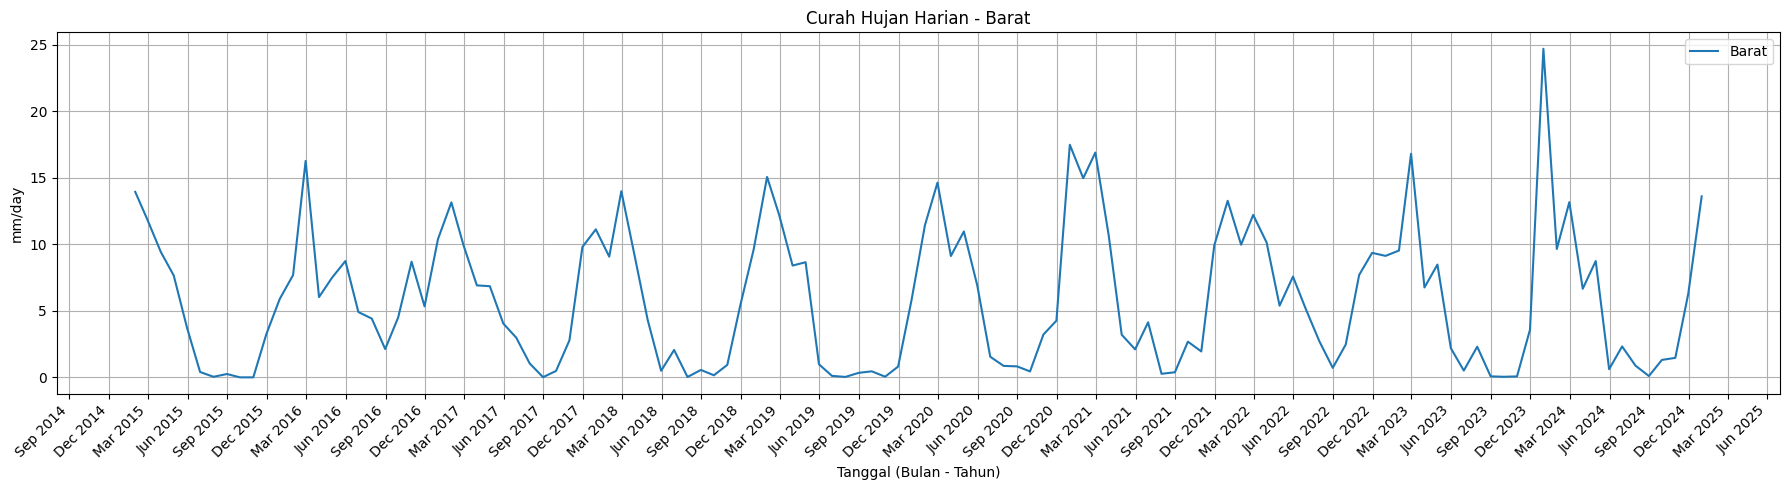
\includegraphics[width=0.9\textwidth]{images/bab_4/curah-hujan-barat.png}
    \caption{Pola Curah Hujan Wilayah Barat}
    \label{fig:pola-curah-hujan-barat}
\end{figure}
Curah hujan harian di Wilayah Barat selama periode 2015–2024 memperlihatkan pola musiman yang sangat jelas, dengan peningkatan intensitas hujan yang konsisten terjadi pada bulan Desember hingga Maret serta kondisi curah hujan rendah hingga mendekati nol pada bulan Juni hingga September. Puncak hujan tahunan umumnya berada pada kisaran 12–18 mm/hari, disertai beberapa kejadian ekstrem yang mencapai lebih dari 20 mm/hari pada tahun-tahun seperti 2017, 2020, 2022, dan 2024. Dengan struktur musiman yang kuat dan variabilitas yang cukup signifikan, deret waktu pada wilayah ini sangat mendukung penerapan model STARIMA dalam mempelajari hubungan spasial-temporal serta memprediksi curah hujan dengan lebih akurat.

\begin{figure}[H]
    \centering
    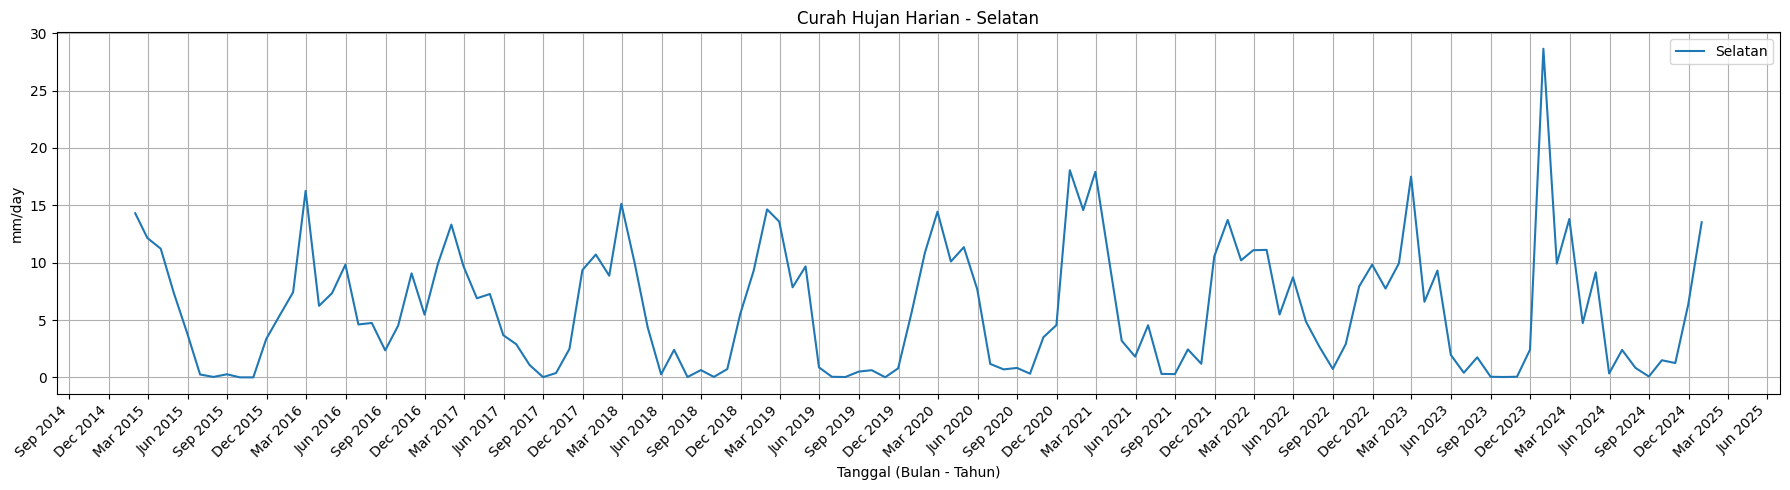
\includegraphics[width=0.9\textwidth]{images/bab_4/curah-hujan-selatan.png}
    \caption{Pola Curah Hujan Wilayah Selatan}
    \label{fig:pola-curah-hujan-selatan}
\end{figure}
Curah hujan harian di Wilayah Selatan selama periode 2015–2024 menunjukkan pola musiman yang sangat konsisten, ditandai dengan peningkatan intensitas hujan pada bulan Desember hingga Maret dan kondisi hampir tanpa hujan pada periode Juni hingga September. Puncak hujan tahunan umumnya berada pada kisaran 12–18 mm/hari, dengan beberapa kejadian ekstrem yang melebihi 20 mm/hari terutama pada awal 2016, 2021, dan 2024. Variabilitas intra-tahunan yang cukup tinggi serta fluktuasi intensitas yang tajam menggambarkan dinamika atmosfer yang aktif di wilayah ini, sekaligus menegaskan adanya komponen musiman yang kuat dan berulang. Pola temporal yang terstruktur ini mendukung penerapan model deret waktu spasial-temporal seperti STARIMA untuk memodelkan dan memprediksi curah hujan secara lebih akurat.

\begin{figure}[H]
    \centering
    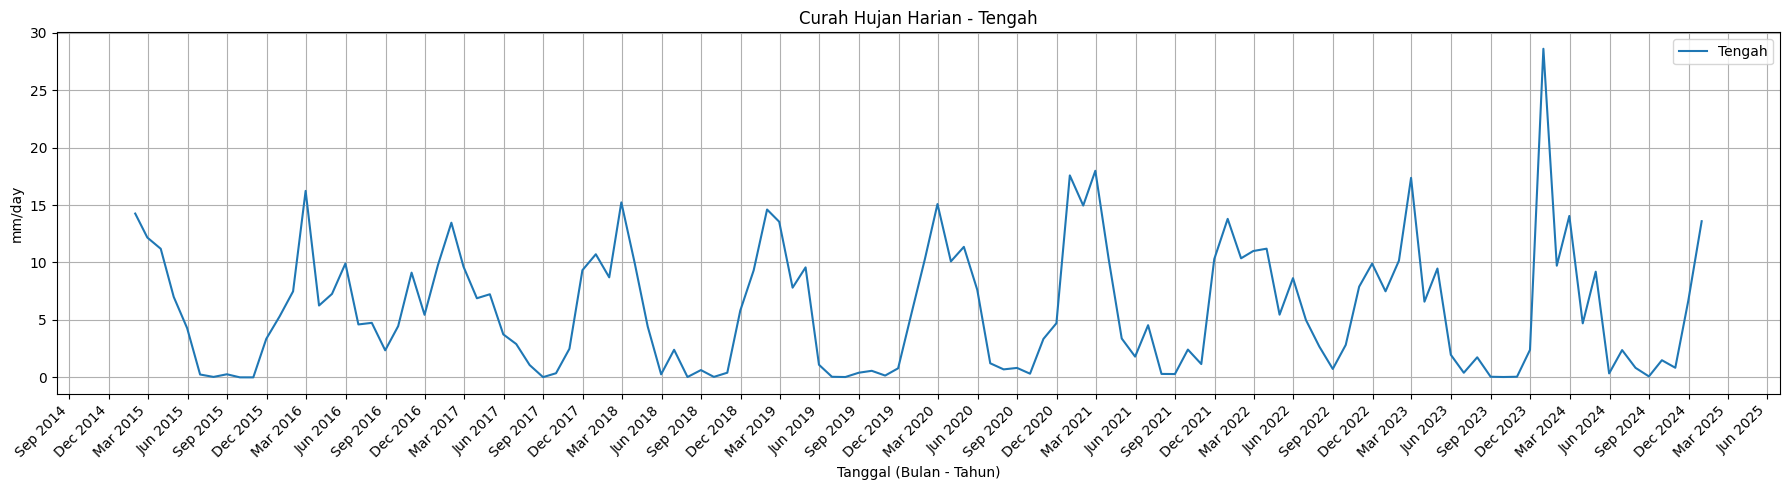
\includegraphics[width=0.9\textwidth]{images/bab_4/curah-hujan-tengah.png}
    \caption{Pola Curah Hujan Wilayah Tengah}
    \label{fig:pola-curah-hujan-tengah}
\end{figure}
Curah hujan harian di Wilayah Tengah selama periode 2015–2024 menunjukkan pola musiman yang sangat jelas, dengan intensitas hujan meningkat secara konsisten pada Desember hingga Maret dan menurun drastis pada Juni hingga September. Variabilitas intra-tahunan tampak cukup tinggi, ditandai dengan fluktuasi tajam antara kondisi tanpa hujan hingga puncak 10–15 mm/hari, serta beberapa kejadian ekstrem seperti pada awal 2024 yang mencapai lebih dari 25 mm/hari. Pola yang stabil dan berulang ini mencerminkan dinamika monsun yang kuat serta pengaruh faktor atmosfer regional yang membentuk variasi hujan tahunan. Struktur temporal yang konsisten tersebut mendukung penerapan model STARIMA dalam memodelkan dan memprediksi curah hujan berbasis hubungan spasial-temporal antar wilayah di Surabaya.

\begin{figure}[H]
    \centering
    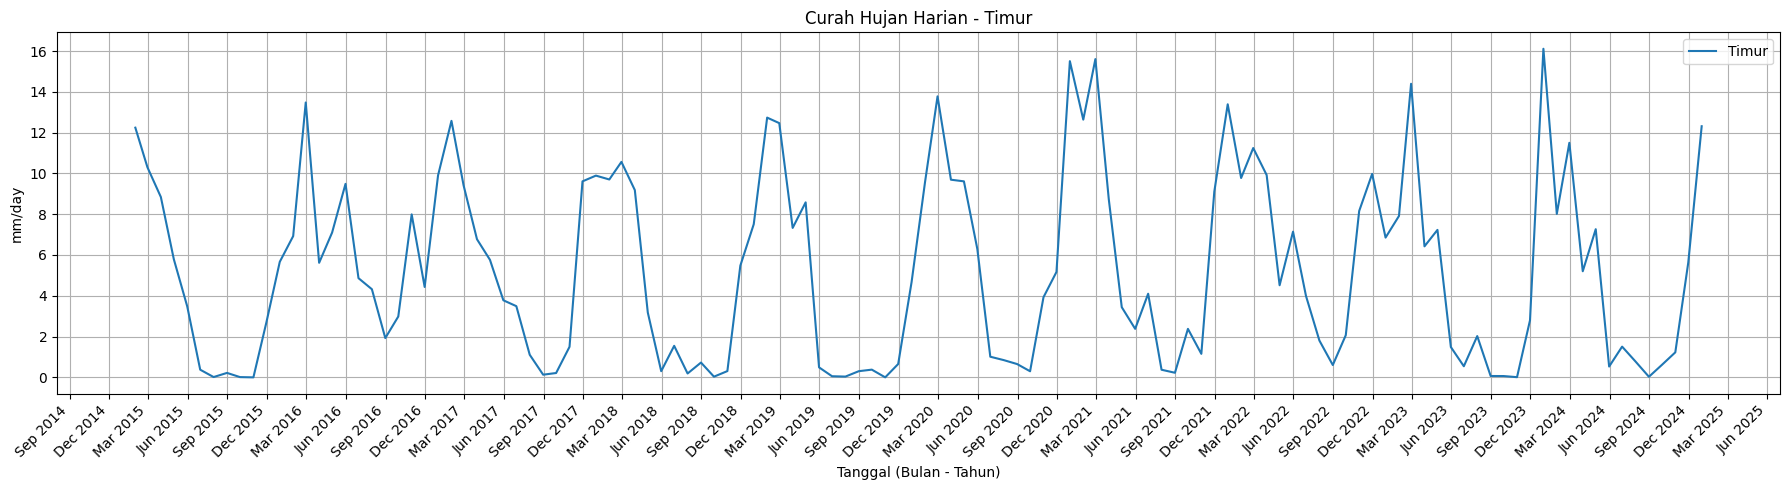
\includegraphics[width=0.9\textwidth]{images/bab_4/curah-hujan-timur.png}
    \caption{Pola Curah Hujan Wilayah Timur}
    \label{fig:pola-curah-hujan-timur}
\end{figure}
Curah hujan harian di Wilayah Timur selama periode 2015–2024 memperlihatkan pola musiman yang konsisten, dengan intensitas hujan meningkat pada bulan Desember hingga Maret dan menurun drastis mendekati nol pada periode Juni hingga September. Puncak hujan tahunan berada pada kisaran 10–15 mm/hari, dengan beberapa kejadian ekstrem yang melampaui nilai tersebut, seperti pada awal tahun 2021, 2022, dan 2024. Fluktuasi intra-tahunan yang tajam dan variasi antar tahun menunjukkan dinamika atmosfer yang aktif di wilayah ini, dipengaruhi oleh siklus monsun dan fenomena cuaca regional. Pola temporal yang berulang dan stabil ini menunjukkan bahwa wilayah Timur memiliki struktur deret waktu yang kuat untuk dimodelkan melalui pendekatan STARIMA dalam analisis spasial-temporal curah hujan.

\begin{figure}[H]
    \centering
    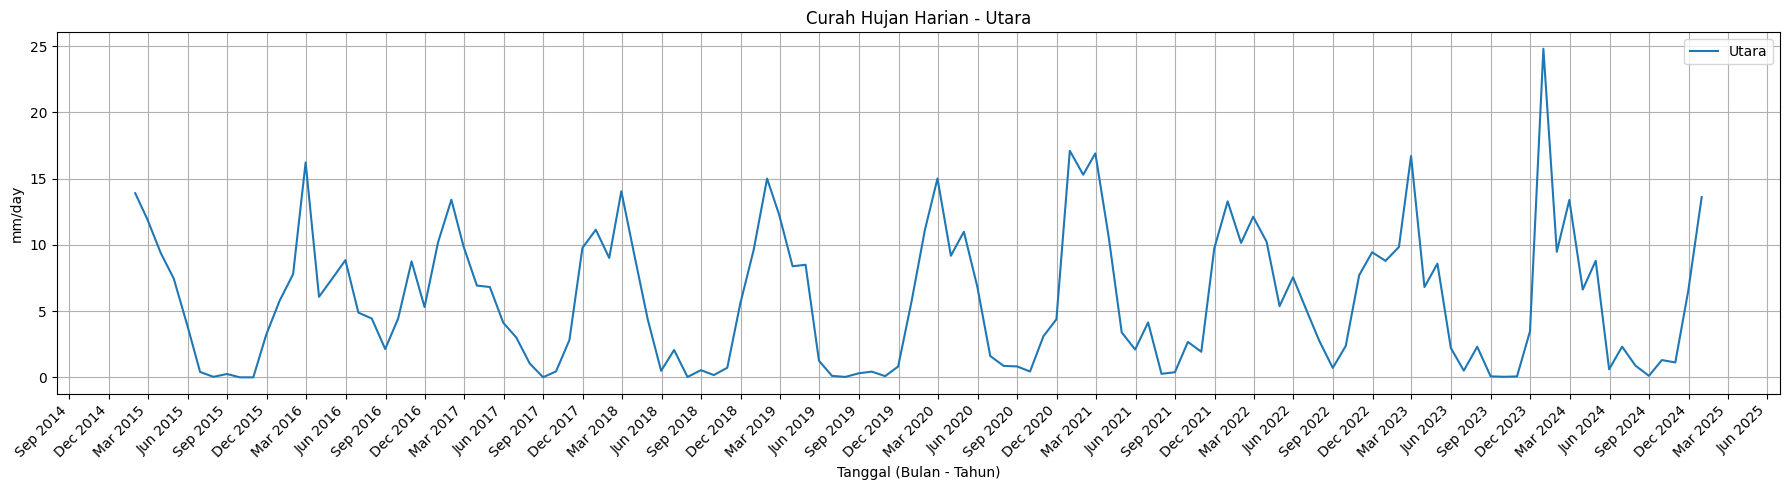
\includegraphics[width=0.9\textwidth]{images/bab_4/curah-hujan-utara.png}
    \caption{Pola Curah Hujan Wilayah Utara}
    \label{fig:pola-curah-hujan-utara}
\end{figure}
Curah hujan harian di Wilayah Utara selama periode 2015–2024 menunjukkan pola musiman yang sangat konsisten, dengan peningkatan intensitas pada bulan Desember hingga Maret dan curah hujan yang hampir nol pada periode Juni hingga September. Puncak hujan tahunan berada pada kisaran 10–15 mm/hari, disertai beberapa kejadian ekstrem yang melebihi 20 mm/hari, terutama pada awal tahun 2020, 2022, dan 2024. Fluktuasi yang tajam antar musim menggambarkan dinamika atmosfer regional yang aktif dan dipengaruhi oleh siklus monsun serta fenomena cuaca skala besar seperti MJO dan ENSO. Pola temporal yang stabil dan berulang ini menunjukkan bahwa Wilayah Utara memiliki struktur deret waktu yang kuat dan cocok dimodelkan menggunakan pendekatan STARIMA untuk analisis dan peramalan spasial-temporal curah hujan.

\subsection{Karakteristik dengan BoxPlot}
Sebelum masuk ke analisis lebih lanjut, diperlukan pemahaman mengenai pola dasar distribusi curah hujan di setiap wilayah. Oleh karena itu, boxplot digunakan untuk menampilkan gambaran awal mengenai sebaran dan karakteristik data curah hujan bulanan.
\begin{figure}[H]
    \centering
    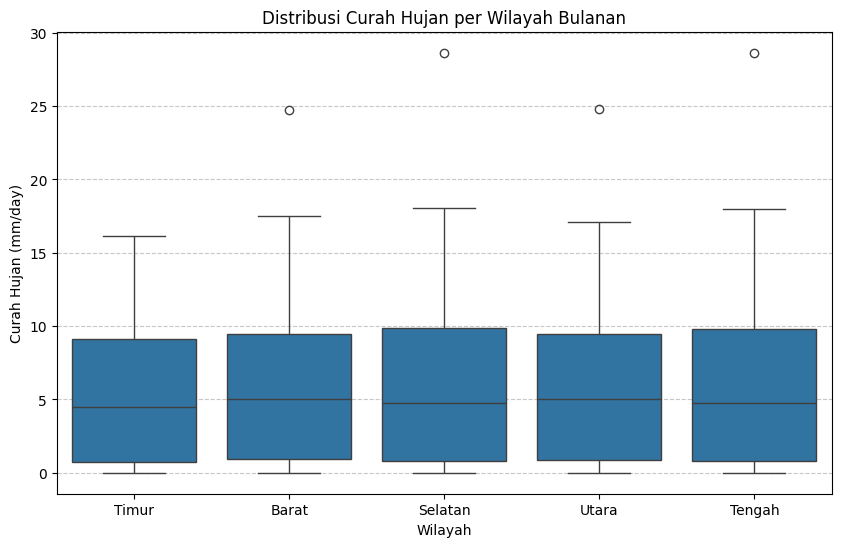
\includegraphics[width=0.9\textwidth]{images/bab_4/boxplot-semua-wilayah.png}
    \caption{Boxplot Kelima Wilayah di Surabaya}
    \label{fig:boxplot-lima-wilayah}
\end{figure}
Gambar \ref{fig:boxplot-lima-wilayah} menampilkan boxplot distribusi curah hujan bulanan untuk lima wilayah di Kota Surabaya, yaitu Timur, Barat, Selatan, Utara, dan Tengah. Secara umum, kelima wilayah menunjukkan pola distribusi yang relatif serupa dengan median curah hujan berada di rata-rata 5 mm/hari, menandakan bahwa sebagian besar nilai curah hujan bulanan terkonsentrasi pada tingkat menengah. Rentang interkuartil (IQR) di seluruh wilayah menunjukkan variasi yang moderat, menggambarkan tingkat sebaran data yang cukup stabil antarwilayah. Meskipun demikian, terlihat adanya beberapa outlier pada Wilayah Barat, Selatan, dan Tengah dengan nilai di atas 25 mm/hari yang menandakan adanya kejadian hujan ekstrem pada periode tertentu. Sementara itu, nilai minimum di setiap wilayah mendekati nol, menunjukkan periode kering yang umum terjadi selama musim kemarau. Tidak terdapat perbedaan yang signifikan antarwilayah dalam hal median maupun rentang variasi, yang mengindikasikan bahwa pola distribusi curah hujan bulanan di Surabaya relatif homogen secara spasial, meskipun dengan sedikit perbedaan amplitudo akibat pengaruh lokal seperti topografi dan kedekatan terhadap kawasan pesisir.

\subsection{Analisis Temporal Curah Hujan}
Analisis temporal dilakukan untuk mengidentifikasi pola perubahan curah hujan dari waktu ke waktu. Berdasarkan grafik deret waktu bulanan yang dibuat untuk masing – masing wilayah terlihat bahwa pola curah hujan Surabaya cenderung musiman dan berulang setiap tahun.
\begin{figure}[H]
    \centering
    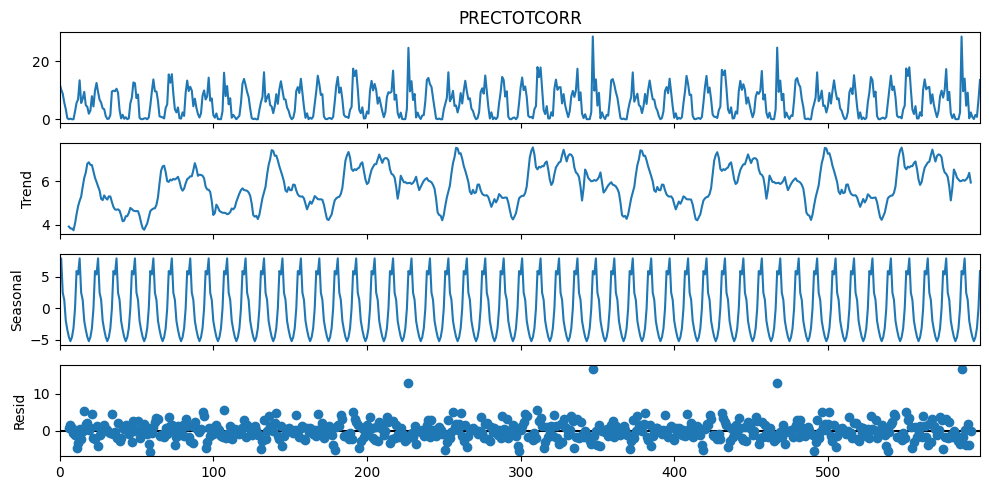
\includegraphics[width=0.9\textwidth]{images/bab_4/seasonal-decompose-semua-wilayah.png}
    \caption{Seasonal Decompose Semua Wilayah}
    \label{fig:seasonal-decompose-semua-wilayah}
\end{figure}

Berdasarkan hasil dekomposi pada gambar \ref{fig:seasonal-decompose-semua-wilayah} tersebut dapat dijelaskan bahwa:
\begin{enumerate}[label=\alph*.]
    \item Komponen Tren:
    
        Pola tren menunjukan adanya fluktuasi jangka panjang yang cenderung meningkat secara perlahan hingga pertengahan periode pengamatan, kemudian relatif stabil. Hal ini mengindikasikan bahwa selama 2015-2024, curah hujan di seluruh wilayah Surabaya mengalami kecenderungan peningkaan moderat  yang mungkin dipengaruhi oleh faktor klimatologis regional.
        
    \item Komponen Musiman:
    
        Pola musiman menunjukkan fluktuasi yang berulang secara konsisten setiap tahun, dengan puncak curah hujan umumnya terjadi pada Desember – Februari dan minimum pada Juli – September. Pola ini menggambarkan dengan jelas siklus tahunan curah hujan di semua wilayah Surabaya yang mengikuti pola iklim monsun tropis.

    \item Komponen Residual:

        Komponen residual menunjukkan penyebaran acak disekitar nol yang menandakan bahwa sebagian besar variasi curah hujan telah berhasil dijelaskan oleh komponen tren dan musiman. Tidak terlihat adanya pola sistematis yang menonjol pada residu, sehingga model dekomposis dianggap cukup baik dalam memisahkan variasi utama pada data
\end{enumerate}

\subsection{Analisis Korelasi Spatio Temporal}
Analisis korelasi spasio-temporal dilakukan untuk mengidentifikasi tingkat keterhubungan pola curah hujan antar wilayah Surabaya.
Nilai korelasi yang ditampilkan pada tabel berikut memberikan gambaran mengenai seberapa kuat kesamaan pola hujan secara ruang dan waktu.

\begin{table}[H]
\centering
\caption{Tabel Korelasi Setiap Wilayah}
\label{table:korelasi-setiap-wilayah}
\begin{tabular}{lccccc}
\hline
\textbf{Wilayah} & \textbf{Barat} & \textbf{Selatan} & \textbf{Tengah} & \textbf{Timur} & \textbf{Utara} \\
\hline
Barat   & 1.000000 & 0.994376 & 0.993769 & 0.983211 & 0.999738 \\
Selatan & 0.994376 & 1.000000 & 0.999631 & 0.975665 & 0.994562 \\
Tengah  & 0.993769 & 0.999631 & 1.000000 & 0.975762 & 0.994531 \\
Timur   & 0.983211 & 0.975665 & 0.975762 & 1.000000 & 0.983363 \\
Utara   & 0.999738 & 0.994562 & 0.994531 & 0.983363 & 1.000000 \\
\hline
\end{tabular}
\end{table}

Tabel~\ref{table:korelasi-setiap-wilayah} merupakan tabel yang menunjukkan bahwa kelima wilayah di Surabaya ini memiliki nilai korelasi yang besar antara 0.975 hingga 0.999.
Korelasi ini menunjukkan hubungan positif yang sangat kuat artinya peningkatan curah hujan di satu wilayah cenderung diikuti oleh peningkatan di wilayah lain pada waktu yang sama.
Hal ini menandakan bahwa curah hujan di Surabaya bersifat homogen secara spasial karena semua wilayah mengalami kondisi meteorologis yang hampir sama.